\section{SVD-VLC System Design}
\label{sec:svdvlc}
\graphicspath{{_System/figures_svdvlc/}}

\subsection{Singular Value Decomposition - Native System}
\label{subsec:svdvlcNative}
The SVD technique applies coordinate system transformations on correlated channels and generates simultaneous independent links and maximizes the capacity of the MIMO channel when the CSI is known at the transmitter and the receiver. The channel matrix $\bf{H}$ can be decomposed into rotation and scaling matrices using SVD as 

\begin{equation}
	\label{eqHsvd}
	\bf{H} = \bf{U}\bf{\Lambda}\bf{V}^{*}
\end{equation}

$\bf{U}$ and $\bf{V}$ are unitary rotation matrices while $\bf{\Lambda}$ is a diagonal scaling matrix. Matrices $\bf{H}$ and $\bf{\Lambda}$ have the same rank $\Gamma\leq min(N_{tx},N_{px})$. The diagonal elements of $\bf{\Lambda}$ $(\lambda_{1}...\lambda_{k}...\lambda_{\Gamma})$ are the singular values of matrix $\bf{H}$ and the squared singular values are the eigenvalues of ${\bf{H}}{\bf{H}}^{*}$. Now let us define new variables in rotated coordinate systems as

\begin{gather}
	\bf{X}^{'} := \bf{V}^{*}\bf{X}\\
	\bf{Y}^{'} := \bf{U}^{*}\bf{Y}\\
	\bf{W}^{'} := \bf{U}^{*}\bf{W}
\end{gather}

Inserting the above definations in MIMO channel model and then pre-multiplying both sides by $\bf{U}^{*}$ transforms the MIMO channel model as

\begin{equation}
	\label{eqSVDChannel}
	\bf{Y}^{'} = \bf{\Lambda}\bf{X}^{'} + \bf{W}^{'}
\end{equation}

\begin{figure}[!t]
	\centering
		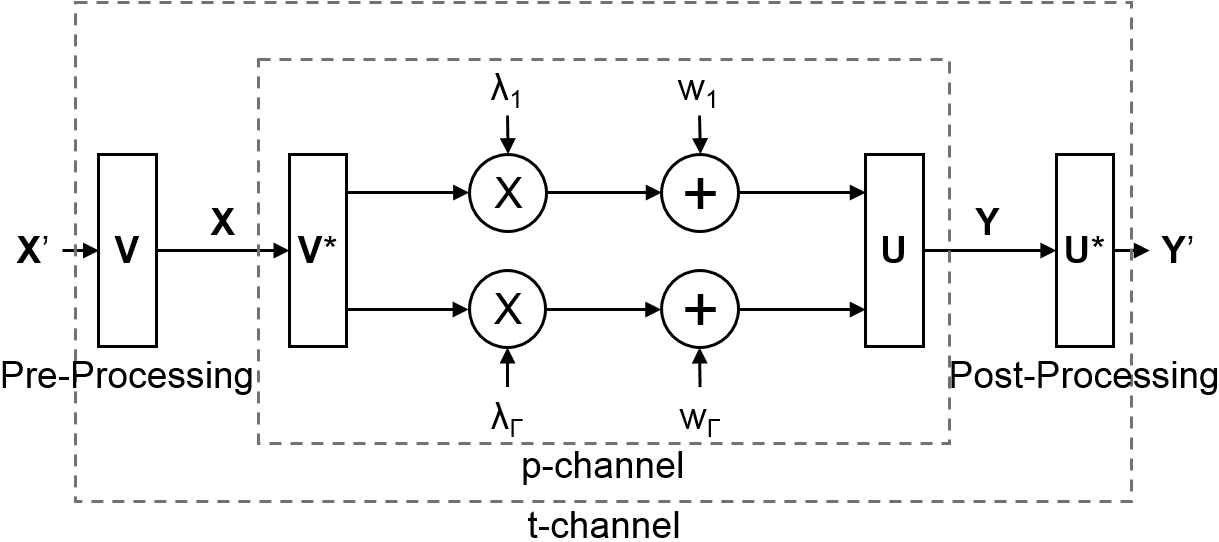
\includegraphics[width=6in]{figSVD.png}
	\caption[Native SVD System Block Diagram]{Native SVD System Block Diagram\footnotemark}
	\label{fig:SVD}
\end{figure}
\footnotetext{Adapted from \cite{tse05a}, pg 292-293}

\figurename{ {\ref{fig:SVD}}} illustrates the transformed MIMO channel. $\bf{X}^{'}$ are the inputs for the data streams in the coordinate system defined by columns of $\bf{V}$ and $\bf{Y}^{'}$ are the outputs in the coordinate system defined by columns of $\bf{U}$. Since $\bf{U}$ is a unitary martix, elements of $\bf{W}^{'}$ will be IID and have the same variance (noise power) as $\bf{W}$ \cite{tse05a}. Since $\bf{\Lambda}$ is a diagonal matrix, extracting the simultaneous equations from Eq.\ref{eqSVDChannel} gives $\Gamma$ simultaneous independent link models described by
 
\begin{equation}
	\label{eqSVDChannel2}
	y^{'}_{k} = \lambda_{k}x^{'}_{k} + w^{'}_{k}; 1\leq{k}\leq\Gamma
\end{equation}

In RF MIMO systems, the aggregate transmit power is the binding constraint. The waterfilling algorithm \cite{gol97a} provides a solution for allocate powers to the independent streams in order to maximize the channel capacity. As a result of this optimization, links with SNR greater than a threshold, are allocated power budget corresponding to their SNRs, while those with SNR below the threshold do not transmit any information. Let ${\bf{K}^{'}_{k}}$ be these waterfilling power allocations. Then the upper bound on the capacity of the channel is given by

\begin{equation}
	\label{eqSVDCap}
	C_{SVD} < \sum_{k=1}^{\Gamma}log_{2}\left(1 + \frac{\lambda_{k}^{2} {K}^{'}_{k}}{\sigma_{MIMO}^{2}B}\right)
\end{equation}

%For a VLC system, the average radiant flux emitted by individual luminaires needs to be maintained to achieve the requested illumination state. These issues are resolved in the SVD-VLC system tackled in the next section.

%%%%%%%%%%%%%%%%%%%%%%%%%%%%%%%%%%%%%%%%%%%%%%%%%%%%%%%%%%%%%%%%
%%%%%%%%%%%%%%%%             SVD-VLC            %%%%%%%%%%%%%%%%
%%%%%%%%%%%%%%%%%%%%%%%%%%%%%%%%%%%%%%%%%%%%%%%%%%%%%%%%%%%%%%%%
\subsection{Singular Value Decomposition - VLC System}
\label{subsec:svdvlcSystem}
In the above model, the information streams are defined over inputs $x^{'}_{k}$. Note $\lambda_{k}=0; k>\Gamma$ and thus no information can be transmitted over those links. At the transmitters, transformation $\bf{V}$ multiplexes the streams over the physical channel. At the receiver,  transformation $\bf{U}^{*}$ demultiplexes the independent streams. These transformations are also called pre-processing and post-processing.

An SVD architecture with different power and offset allocation has been proposed for MIMO VLC communications in \cite{par11a}. In this work, the aggregate sum of average radiated optical flux from multiple LEDs is constrained to be smaller than or equal to an upper bound in order to fulfill the eye safety requirements. Under this condition, it is still possible for the system to inadvertently violate the eye safety limit if the channel matrix is not full rank despite satisfying the stated constraints. Alternately, the system will under-utilize the capacity of the channel. Also, the illumination generated by that system changes with the channel matrix thus transitioning to a different illumination state every time the channel matrix is changed. Finally, the solution restricts itself to M-PAM and necessitates different optimization for different modulation schemes.

Native SVD does not impose any form of non-negativity or illumination constraint. The SVD-VLC architecture is derived from the native SVD architecture to optimally utilize the capacity of the channel while satisfying illumination constraints. For indoor VLC system to provide illuminaion and optical wireless access simultaneously, the channel constraints are given by

\subsubsection{Non-Negativity Constraint}
\label{subsubsec:svdvlcSystemNonnegative}

For indoor VLC system, information is carried over an intensity signal which cannot be negative. \ref{eqConsNN} implies that input symbols should be defined to generate positive values after preprocessing.
\begin{equation}
	\label{eqConsNN}
	{\bf{X}} \geq {\bf{0}} \leftrightarrow {\bf{V}}{\bf{X}}^{'} \geq {\bf{0}}\\
\end{equation}
	
\subsubsection{Illumination Constraint}
\label{subsubsec:svdvlcSystemIllumination}

In an indoor space, a user can specify a desired illumination state. This specifies the average radiant flux to be emitted by each luminaire. Eq.\ref{eqConsIll} states that the average radiant flux transmitted by each luminaire must equal the desired illumination state. Let ${\bf{P}}$ be the vector that defines the average output radiant flux from each transmitter. Then ${\bf{P}}^{'}$ gives this constraint on the transformed links. This implies that the average signal value in the transformed space must be equal to the corresponding element of ${\bf{P}}^{'}$. 

\begin{equation}
	\label{eqConsIll}
	E[{\bf{X}}] = {\bf{P}} \leftrightarrow {\bf{P}}^{'} = E[{\bf{X}}^{'}] = {\bf{V}}^{*}{\bf{P}}
\end{equation}

It is worth noting that ${\bf{X}}^{'}$ must satisfy the equation for all its elements irrespective of the channel gain of the corresponding transformed link. This implies that when the channel matrix {\bf{H}} or ${\bf{\Lambda}}$ is not full rank, the SVD-VLC architecture still expects the transformed links whose channel gain $\lambda_{k} = 0$ to maintain an average signal level as specified by this constraint. So even though these transformed links carry no information, it is vital to satisfy the average signal constraint to service illumination.

\subsubsection{Input Signal Ranges}
\label{subsubsec:svdvlcSystemRange}

Eq.\ref{eqConsSig} specifies the set of values that ${\bf{X}}^{'}$ can take at any given instant of time provided the other constraints are satisfied.
	\begin{equation}
	\label{eqConsSig}
	M[{\bf{X}}^{'}.sgn({\bf{P}}^{'})] \geq {\bf{0}}
\end{equation}

The above constraint states that the modulated signal for each luminaire can span either the non-negative or the non-positive but not both ranges of the Real number line as dictated by the illumination constraint.

\subsubsection{SVD-VLC Architecture}
\label{subsubsec:svdvlcSystemArchitecture}

\begin{figure}[!t]
	\centering
		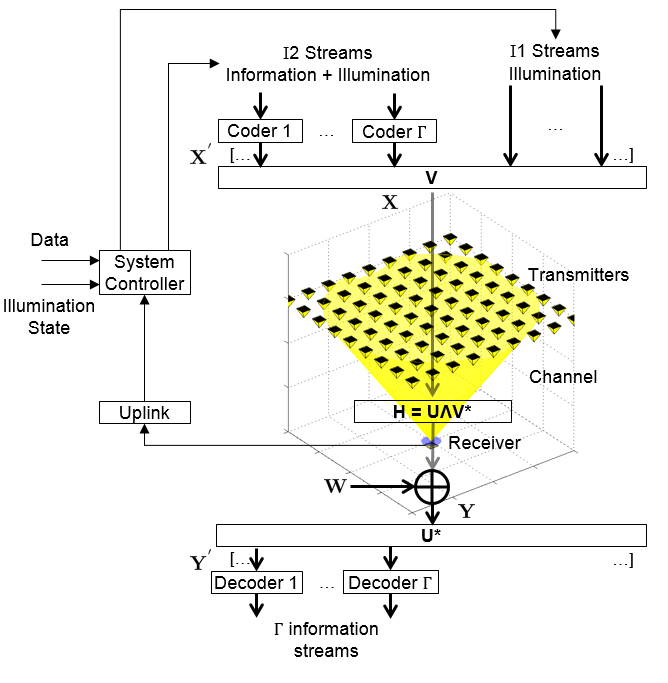
\includegraphics[width=5in]{figSVDVLCblock.png}
	\caption{SVD-VLC System Block Diagram}
	\label{fig:SVDVLCblock}
\end{figure}

\figurename{ \ref{fig:SVDVLCblock}} illustrates SVD-VLC system architecture. The 'I1-streams' are the $N_{tx} - \Gamma$ links that service only illumination. The 'I2-streams' are the $\Gamma$ information $+$ illumination bearing links. The I1 and I2 streams are preprocessed by ${\bf{V}}$ to transform and multiplex them over the channel. This multiplexing generates and maintains the desired illumination state in the indoor space. At the imaging receiver, the TIAs for each pixel add i.i.d white gaussian noise to each link. Postprocessing by ${\bf{U^{*}}}$ demultiplexes the parallel links and recovers the $\Gamma$ I2 streams. The streams can be jointly decoded to optimally recover the transmitted data. Thus the SVD-VLC architecture services the illumination while achieving high data rates over the VLC channel. 

%Thus the SVD-VLC architecture maximizes the achievable data rates over the VLC channel while servicing the illumination mission. The lower bound on capacity of the MIMO VLC channel with imaging receiver can now be derived from Eqs. \ref{eqMimoSNR}, \ref{eqMimoCap} and \ref{eqSVDChannel2} as
%
%\begin{equation}
	%\label{eqSVDCap}
	%C_{SVD-VLC} = \sum_{k=1}^{\Gamma}log_{2}(1 + \frac{\lambda_{k}^{2}{P}_{k}^{'2}}{\sigma_{MIMO}^{2}B})
%\end{equation}

The SVD architecture assumes that the CSI is known at the transmitter and the receiver. For my dissertation, I will investigate MIMO strategies when CSI is not known at transmitter. I also wish to analyze the capacity of the system when each luminaire has a maximum signal power constraint and peak amplitude constraints while maintaining illumination. The receiver can estimate the channel using pilot signals. I also propose the extend the SVD-VLC architecture to support mobile receivers and multiple users.

%%%%%%%%%%%%%%%%%%%%%%%%%%%%%%%%%%%%%%%%%%%%%%%%%%%%%%%%%%%%%%%%
%%%%%%%%%%%%%%%%             RESULTS            %%%%%%%%%%%%%%%%
%%%%%%%%%%%%%%%%%%%%%%%%%%%%%%%%%%%%%%%%%%%%%%%%%%%%%%%%%%%%%%%%
\subsection{Analysis}
\label{sec:analysis}

\begin{table}[!b] %top [!b] bottom
\begin{threeparttable}[b]
\caption{VLC System Configuration Parameters}
\label{tblSystem}
\centering
	\begin{tabular}{|l|c|c|c|}
		\hline
		\multicolumn{2}{|c|}{\bf{Parameter}} & \bf{Value} & \bf{Units}\\
		\hline
		Room Length & $L_{rm}$ & 4 & m\\
		\hline
		Room Width & $W_{rm}$ & 4 & m\\
		\hline
		Room Height & $H_{rm}$ & 4 & m\\
		\hline
		Transmiter grid pitch\tnote{1} & $D_{tx}$ & 0.5 & m\\
		\hline
		Total number of transmitters\tnote{1} & $N_{tx}^{L}$ x $N_{tx}^{W}$ & 9x9 & -\\
		\hline
		Transmitter Lambertian Order & $m$ & 1 & -\\
		\hline
		Optics Field of View & $\psi_{c}^{o}$ & 60 & degrees\\
		\hline
		Optics focal length\tnote{1} & $f$ & 5 & mm\\
		\hline
	  Optics transmission\tnote{1} & $Q$ & 1 & -\\
		\hline
		Concentrator refractive index\tnote{2} & $\eta$ & 1.5 & -\\
		\hline
		Ideal filter transmission & $T(\lambda)\forall \lambda$ & 1 & -\\
		\hline
		Sensor Side length & $a_{rx}$ & 5 & mm\\
		\hline
		Pixel side length\tnote{1} & $\alpha_{rx}$ & 1 & mm\\
		\hline
		Pixel pitch\tnote{1} & $\delta_{rx}$ & 1 & mm\\
		\hline
		Total number of pixels\tnote{1} & $N_{px}^{L}$ x $N_{px}^{W}$ & 5x5 & -\\
		\hline
		Responsivity & $R(\lambda)\forall \lambda$ & 0.4 & A/W\\
		\hline
		Receiver bandwidth & $B$ & 50 & MHz\\
		\hline
		TIA noise current density & $I_{pa}$ & 5 & pA/$\sqrt{\text{Hz}}$\\
		\hline
	\end{tabular}
	\begin{tablenotes}
	\item [1] MIMO specific parameter
	\item [2] SISO specific parameter
	\end{tablenotes}
	\end{threeparttable}
\end{table}

The capacity of the MIMO channel with imaging receiver is analyzed and compared with an equivalent SISO channel. Table \ref{tblSystem} outlines the system parameters used. For the MIMO channel, the luminaires are arranged in a grid at the a height of 3m in the room and at a pitch of $D_{tx}$. The luminaires are assumed to be point sources with enough output luminous flux to provide the desired illumination. The SPD of the emitted flux is approximated using sum of gaussians to that used in \cite{gru08b}. The receiver bandwidth is assumed to be 50 MHz \cite{zen08a}. For this analysis the receiver is always assumed located at the center of the length-width plane. The same sensor side length $a_{rx}$ is maintaied for the SISO PD and the imaging receiver. The case where the aperture collection area of the imaging receiver is the same as the area of the SISO receiver is also considered. 

\begin{figure}[!t]
	\centering
		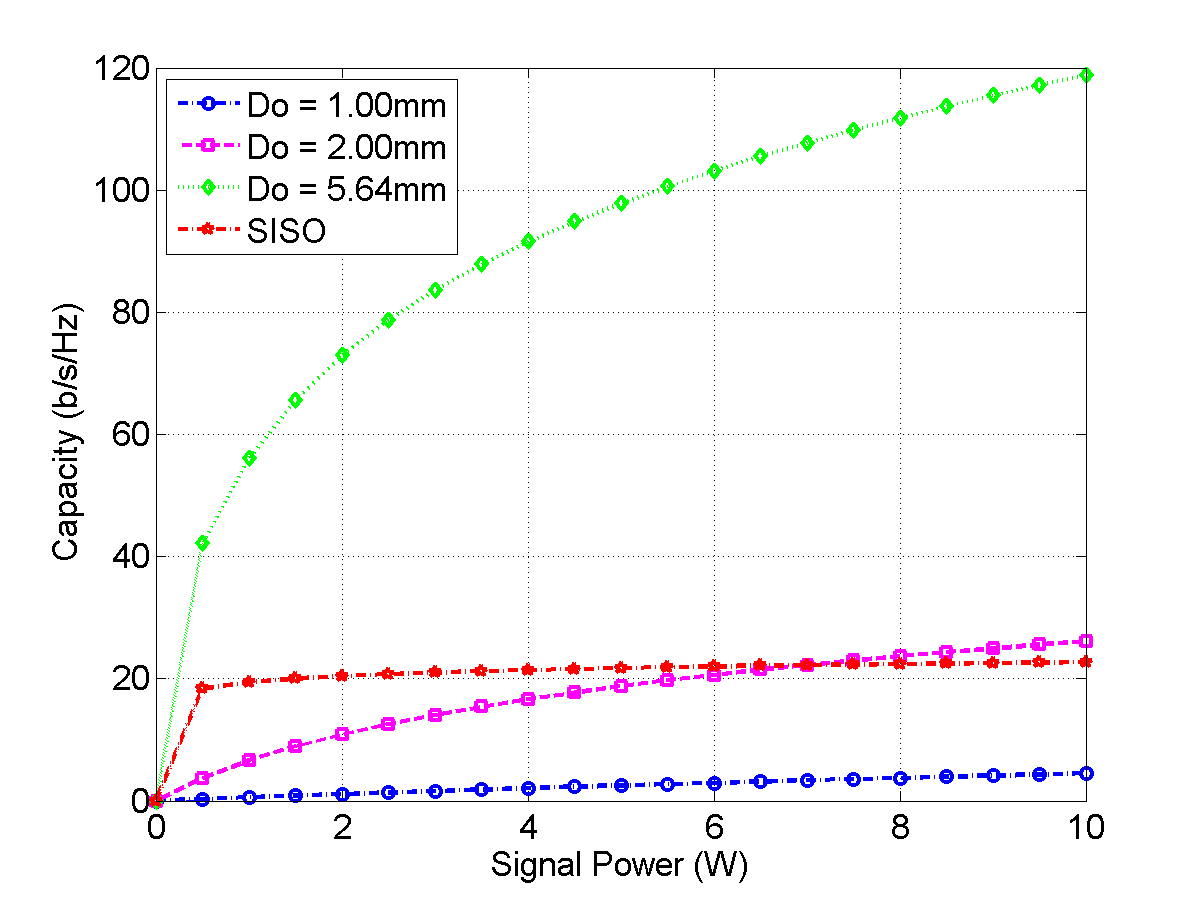
\includegraphics[width=5in]{fig_CapvsPwrvsAp2.png}
	\caption{Capacity vs Dimming}
	\label{figCapVsPwr}
\end{figure}

\figurename{\ref{figCapVsPwr}} shows the theoretical capacity of the SISO and MIMO channels over a range of signal power constraints and different lens aperture diameters when the receiver is at the center of the 1m plane. The capacity of the MIMO VLC channel is then calculated at the same power constraints as a SISO channel. As expected, the capacity of the imaging channel does increase with increasing aperture diameter. At aperture diameter of 5.64mm, the imaging receiver and the SISO receiver collect the same amount of average radiant flux, however the MIMO channel shows hugh spectral efficiency gains. This gain in capacity can be explained by the introduction of multiple parallel links due to the imaging receiver architecture and the reduction in ambient shot noise per channel as indicated in \cite{dja00a}. While the imaging receiver collects the same amount of ambient flux as the SISO receiver, this flux can be assumed to be equally divided among all the pixels on the receiver due to imaging optics. Thus each link has greatly reduced ambient flux, thus reducing the noise and improving the capacity. The limiting factor in this case is the thermal noise.

\begin{figure}[!t]
	\centering
		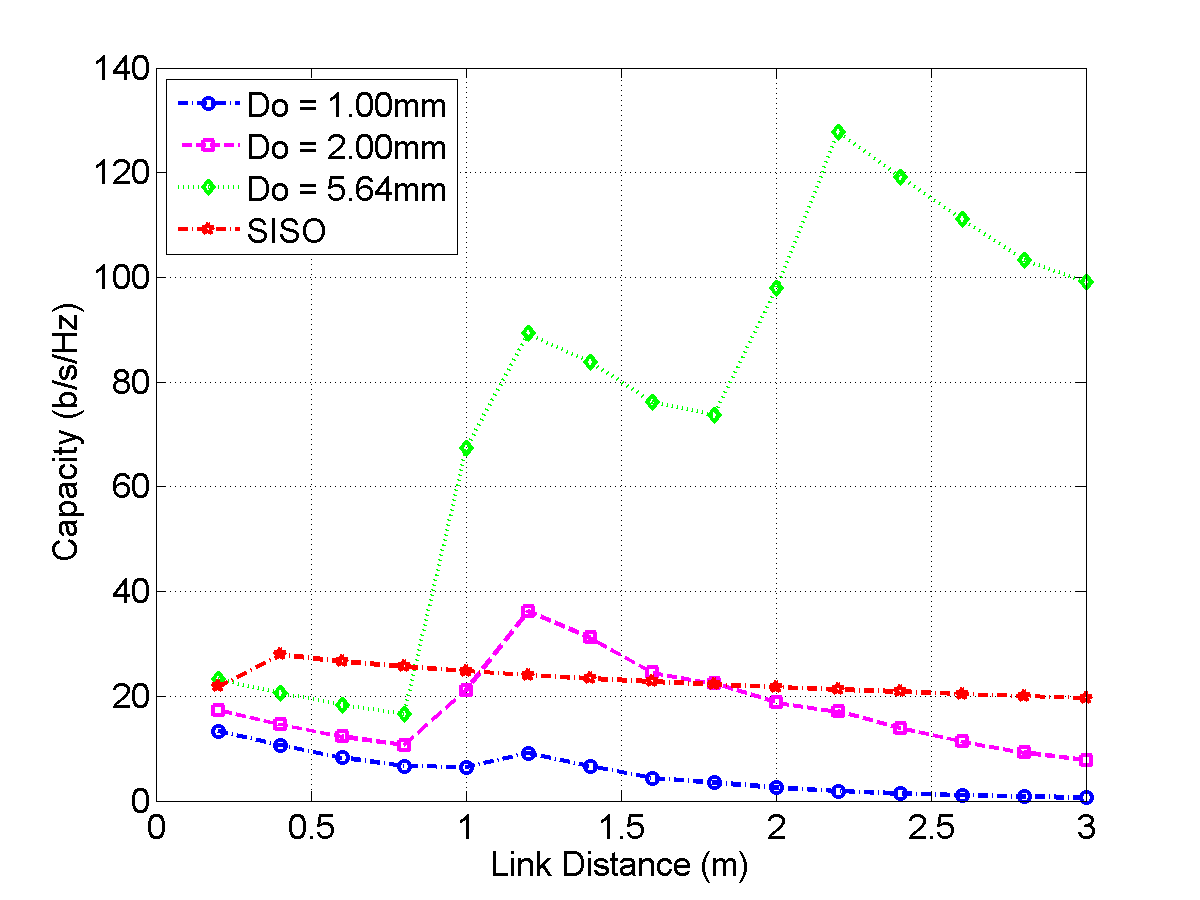
\includegraphics[width=5in]{fig_CapvsLinkvsAp2.png}
	\caption{Capacity vs Link Distance}
	\label{figCapVsLkD}
\end{figure}

\figurename{ \ref{figCapVsLkD}} shows capacities calculated at different link distances when the total signal power is 5W. The link distance here is defined as the length of a vector from origin of the receiver coordinate system along {$\bf{\hat{z}}$} when it intersects the transmitter plane. The SISO channel capacity monotonically decreases with increasing link distance. The capacity of the MIMO channel goes through regions of positive (increasing) and negative (decreasing) slopes. 

\begin{figure}[!t]
	\centering
		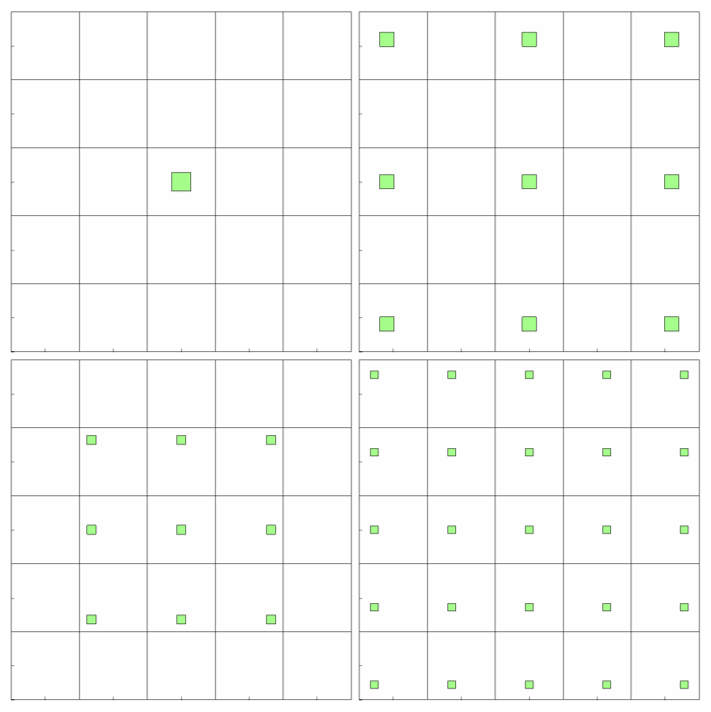
\includegraphics[width=3.5in]{fig_SpotsAtLnkDist.png}
	\caption[Spots on sensor at different link distances]{Spots (magnified for better illustration) as projected on the imaging receiver sensor plane at different link distances which are (a) top left: 1.0m (b) top right: 1.2m (c) bottom left: 2.0m (d) bottom right: 2.2m}
	\label{figSpotsVsLink}
\end{figure}

As seen in \figurename{ \ref{figSpotsVsLink}}a, at the 1m link distance, only 1 transmitter is in the receiver's FOV while adjascent transmitters are just outside the FOV. Increasing the link distance to 1.2m causes the adjascent transmitters to enter the receiver FOV, increasing the number of parallel channels as seen in \figurename{\ref{figSpotsVsLink}}b. The corresponding increase in capacity is greater than the small decrease caused by the increasing link distance. Thus the MIMO channel capacity curve has a positive slope upto 1.2m. Between 1.2m  to 1.8m, number of transmitters seen by receiver remain the same as the link distance is further increased. This causes the capacity of each individual link to decrease thus causing an overall decrease in the channel capacity from 1.2m to 1.8m. \figurename{\ref{figSpotsVsLink}}c shows the transmitters projected on the receiver at a link distance of 2.0m where one can see more adjascent transmitters begin to enter the receiver FOV and at 2.2m as in \figurename{ \ref{figSpotsVsLink}}d, the transmitters are completely in the receiver FOV thus causing an increase in capacity due to more parallel channels. From 2.2m to 2.8m, no more transmitters enter the receiver FOV and thus the overall capacity decreases with increasing link distance. 

Having studied the effect of total power constraint and link distance on the capacities of optical channel with imaging receiver, I wish to study the effect of constraints that the receiver orientation poses on the system performance. Also, as the number of receive pixels increases, so does the need for parallel channels to receive simultaneous streams thus making the receiver more complex. I shall investigate modulation schemes like Spatial Modulation that can benefit from multiple transmitters but reduce the receiver complexity.

\begin{table}[!t] %top [!b] bottom
\caption{SVD-VLC Simulation Illumination Constraints}
\label{tblSimulation}
\centering
	\begin{tabular}{|c|c|c|}
		\hline
		{\bf{Case}} & \bf{Dominant luminaire(s)} & \bf{400lx Setpoint location}\\
		\hline
		a & [1 3 3]' & [1 3 1]'\\
		\hline
		b & [3 1 3]' & [3 1 1]'\\
		\hline
		c & [1 1 3]' and [3 3 3]' & [2 2 1]'\\
		\hline
	\end{tabular}
\end{table}

\begin{table}[!b] %top [!b] bottom
\caption{SVD-VLC Simulation Illumination Results}
\label{tblSimulation2}
\centering
	\begin{tabular}{|c|c|c|c|c|}
		\hline
		\multicolumn{2}{|c|}{\bf{Receiver}} & \multicolumn{3}{|c|}{\bf{Simulated illumination (lx)}}\\
		\hline
		{\bf{Location}} & {\bf{Rank($H$)}} & {\bf{a}} & {\bf{b}} & {\bf{c}}\\
		\hline
		[1.6 0.6 1.0]' & 16 & 399.99 & 400.29 & 400.22\\
		\hline
		[2.8 0.4 1.4]' & 12 & 400.00 & 401.75 & 400.00\\
		\hline
		[0.2 0.8 1.0]' & 12 & 399.81 & 399.92 & 401.26\\
		\hline
		[1.2 1.4 1.6]' & 9 & 400.06 & 400.01 & 401.97\\
		\hline
	\end{tabular}
\end{table}

To  illustrate generation and maintenance of an illumination state using the SVD-VLC architecture, three different scenarios for different illumination states were simulated using SVD-VLC. For these scenarios, the uniform illumination constraint that was relaxed. Table \ref{tblSimulation} now outlines the new illumination constraints. The dominant luminaire(s) column specifies the transmitter(s) whose average output radiant flux  was configured to be 20x that as compared to each of the other transmitters. Setpoint location column specifies the location in the room where 400lx illumination is requested. The combination of these two values specifies a unique illumination state for each scenario. The constraints were specified in this manner to prevent an unacceptably high illumination level at any other point on the illumination surface. A more complex illumination state can be imposed as a constraint to generate a particular light field, however this simple case is sufficient to illustrate the SVD-VLC behavior.

Receiver locations at four different time instants are chosen pseudorandomly to simulate a varying channel matrix due to mobility. For each of the three scenarios, a 1024 length long data sequence was generated from a uniform distributed pseudorandom number sequence in the (0,1) range. The data sequence was scaled to meet the average signal constraint specified by ${\bf{P}}^{'}$ and I1 and I2 streams were generated. After multiplexing these streams over the p-channel, the resulting illumination state was calculated as illustrated in \figurename{ \ref{figIllSVD}}. Table \ref{tblSimulation2} shows values for the illumination achieved at the setpoint location as the channel matrix varies with the receiver's location. It can be seen that despite the variations in the channel matrix, the illumination state remains nearly constant.

\begin{figure}[!t]
	\centering
		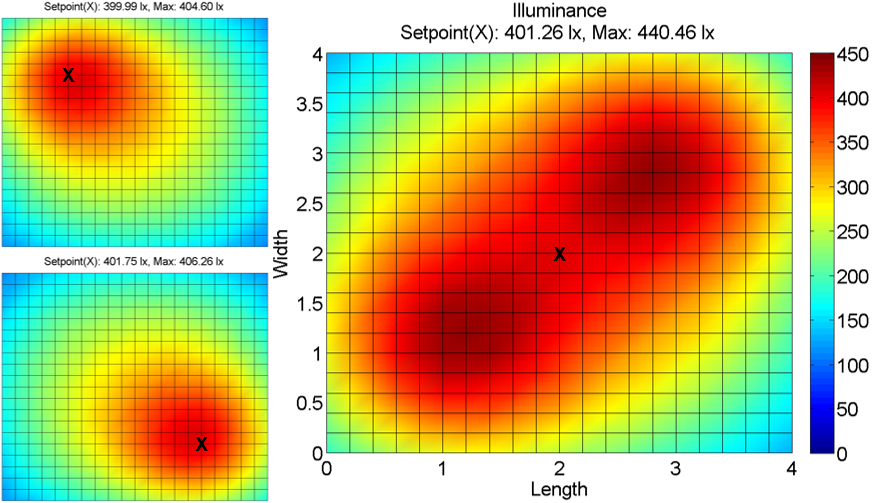
\includegraphics[width=5.5in]{fig_SVDVLC_Ill_full.png}
	\caption[Generation and maintenance of illumination state by SVD-VLC]{Generation and maintenance of illumination state by SVD-VLC. 'X' marks the setpoint location in the illumination plane at 1m height. Scenarios: (a) Top left (b) Bottom left (c) Right }
	\label{figIllSVD}
\end{figure}

